\documentclass{beamer}

\usefonttheme{professionalfonts} % using non standard fonts for beamer
\usefonttheme{serif} % default family is serif

\usepackage{hyperref}

%\usepackage{minted}

\usepackage{animate}

\usepackage{graphicx}

\def\Put(#1,#2)#3{\leavevmode\makebox(0,0){\put(#1,#2){#3}}}

\usepackage{color}

\usepackage{tikz}

\usepackage{amssymb}

\usepackage{enumerate}


\newcommand\blfootnote[1]{%

  \begingroup

  \renewcommand\thefootnote{}\footnote{#1}%

  \addtocounter{footnote}{-1}%

  \endgroup

}

\makeatletter

%%%%%%%%%%%%%%%%%%%%%%%%%%%%%% Textclass specific LaTeX commands.

 % this default might be overridden by plain title style

 \newcommand\makebeamertitle{\frame{\maketitle}}%

 % (ERT) argument for the TOC

 \AtBeginDocument{%

   \let\origtableofcontents=\tableofcontents

   \def\tableofcontents{\@ifnextchar[{\origtableofcontents}{\gobbletableofcontents}}

   \def\gobbletableofcontents#1{\origtableofcontents}

 }

%%%%%%%%%%%%%%%%%%%%%%%%%%%%%% User specified LaTeX commands.

\usetheme{Malmoe}

% or ...

\useoutertheme{infolines}

\addtobeamertemplate{headline}{}{\vskip2pt}



\setbeamercovered{transparent}

% or whatever (possibly just delete it)

\makeatother

\begin{document}
\title[DCEL report]{Parallel DCEL Construction Report}
\author[AC]{Andres Calderon}
\institute[Summer'19]{University of California, Riverside}
\makebeamertitle
\newif\iflattersubsect

\AtBeginSection[] {
    \begin{frame}<beamer>
    \frametitle{Outline} 
    \tableofcontents[currentsection]  
    \end{frame}
    \lattersubsectfalse
}

\AtBeginSubsection[] {
    \begin{frame}<beamer>
    \frametitle{Outline} 
    \tableofcontents[currentsubsection]  
    \end{frame}
}

\begin{frame}{Records in the DCEL construction}
    \begin{itemize}
        \item Vertex(x: Double, y: Double, edge: Half-edge)
        \item Half-edge(origen: Vertex, twin: Half-edge, next: Half-edge, prev: Half-edge, face: Face)
        \item Face(egde: Half-edge, label: String)
    \end{itemize}
\end{frame}

\begin{frame}{DCEL construction outline}
    \begin{itemize}
        \item Input: Set of polygons.
        \item Output: Dataset of Half-edge records
        \begin{enumerate}
         \item Read set of polygons
         \item Partition set of polygons according to a grid
         \item For each partition extract its MBR polygon and clip the polygons inside each partition
         \item For each polygon at each partiion:
            \begin{enumerate}
             \item Extract set of vertices
             \item Create half-edges for each vertex (Algorithm 2)\footnote{Algorithm 2 follows the logic from \url{https://tinyurl.com/y58xk82e}}
            \end{enumerate}
        \item Merge half-edges from each partition
        \end{enumerate}
    \end{itemize}
\end{frame}

\begin{frame}{Algorithm 2}
    \begin{itemize}
        \item Input: Set of vertices.
        \item Output: List of Half-edge records
        \begin{enumerate}
         \item Create lists for Vertex, Half-edge and Face records
         \item Create a Face record for this set of vertices
         \item Set Half-edge records prevLeft and prevRight to null 
         \item For each vertex in vertices:
            \begin{enumerate}
             \item Create a Vertex record from the vertex. 
             \item Create two Half-edge records (left and right) and add to the Half-edge list
             \item Update the the Vertex record and add to the Vertex list
             \item Set the previous next edge to this left edge, Set the previous right edge origen to this vertex
             \item Update prevLeft and prevRight Half-edges to left and right  
            \end{enumerate}
         \item Update the initial Half-edges from the Half-edges list
         \item Update the Face record with one of the Half-edges from the list
        \item Merge half-edges from each partition
        \end{enumerate}
    \end{itemize}
\end{frame}


\begin{frame}{DCEL construction example}
    \centering 
    Set of polygons \\
    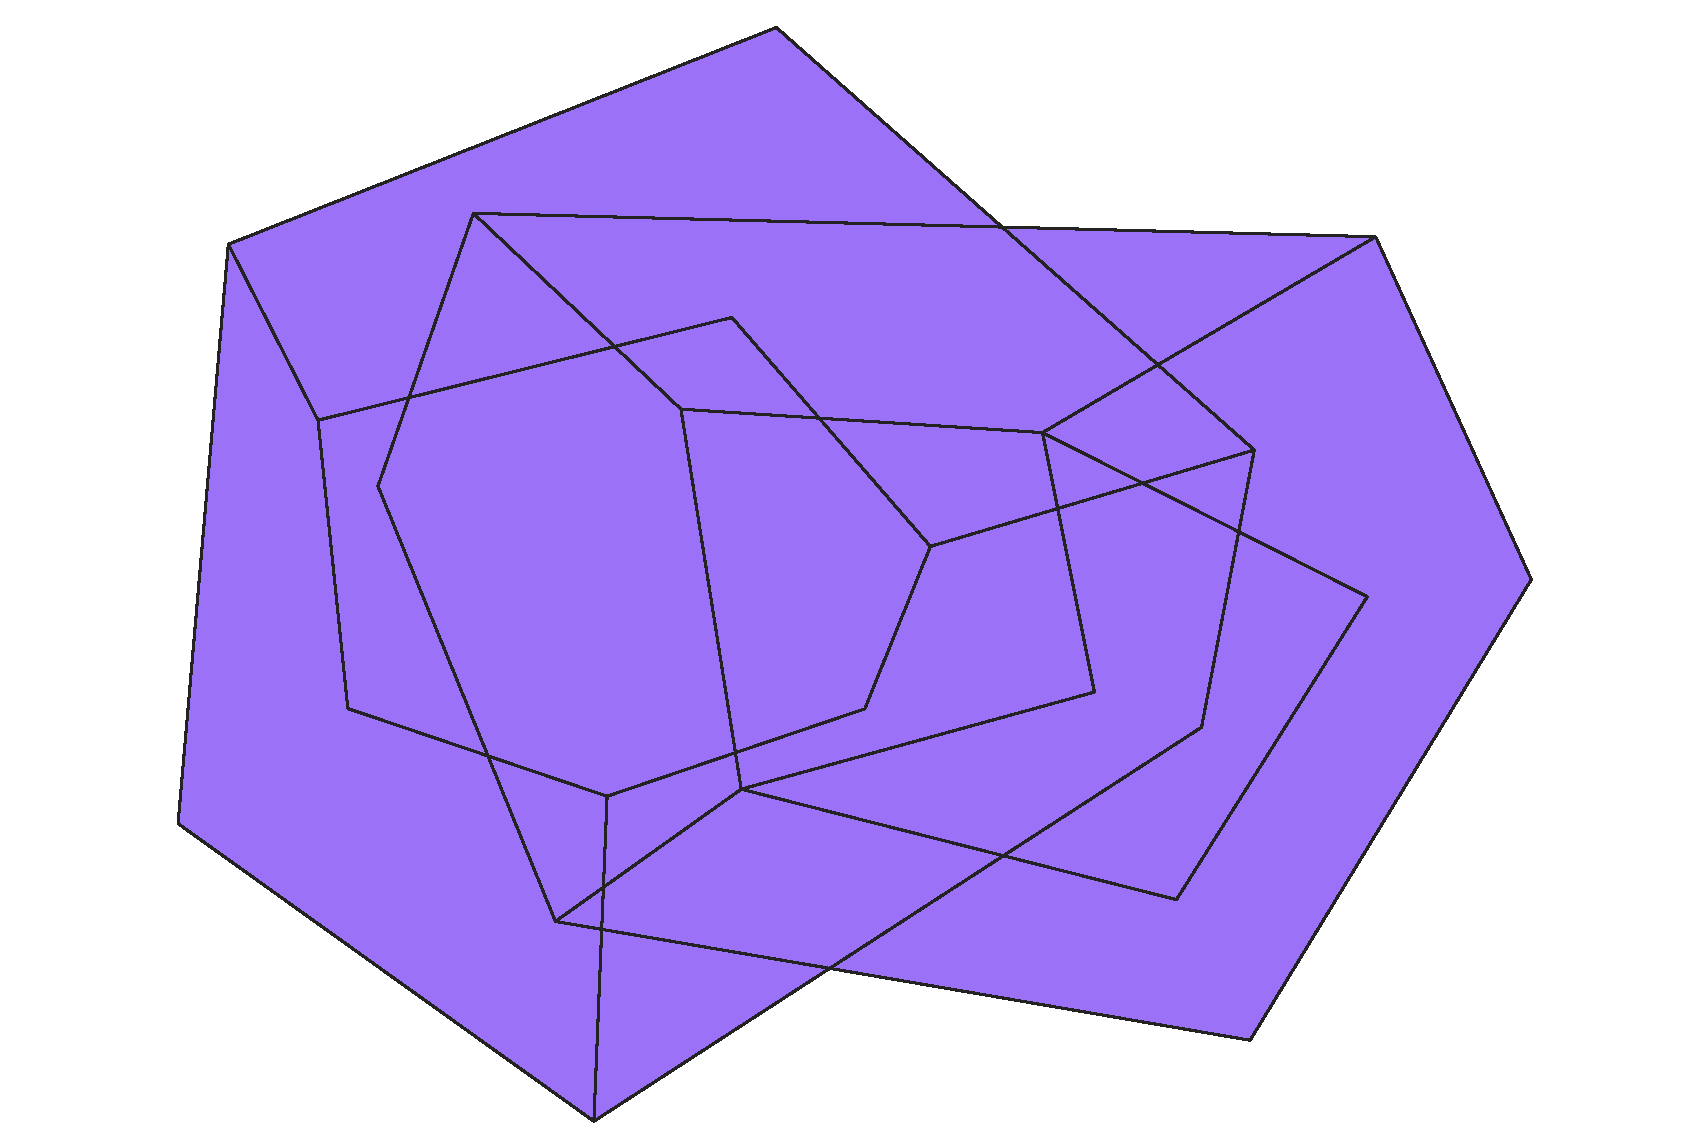
\includegraphics[width=0.8\linewidth]{figures/DCEL01_input} 
\end{frame}

\begin{frame}{DCEL construction example}
    \centering 
    Partitioning \\
    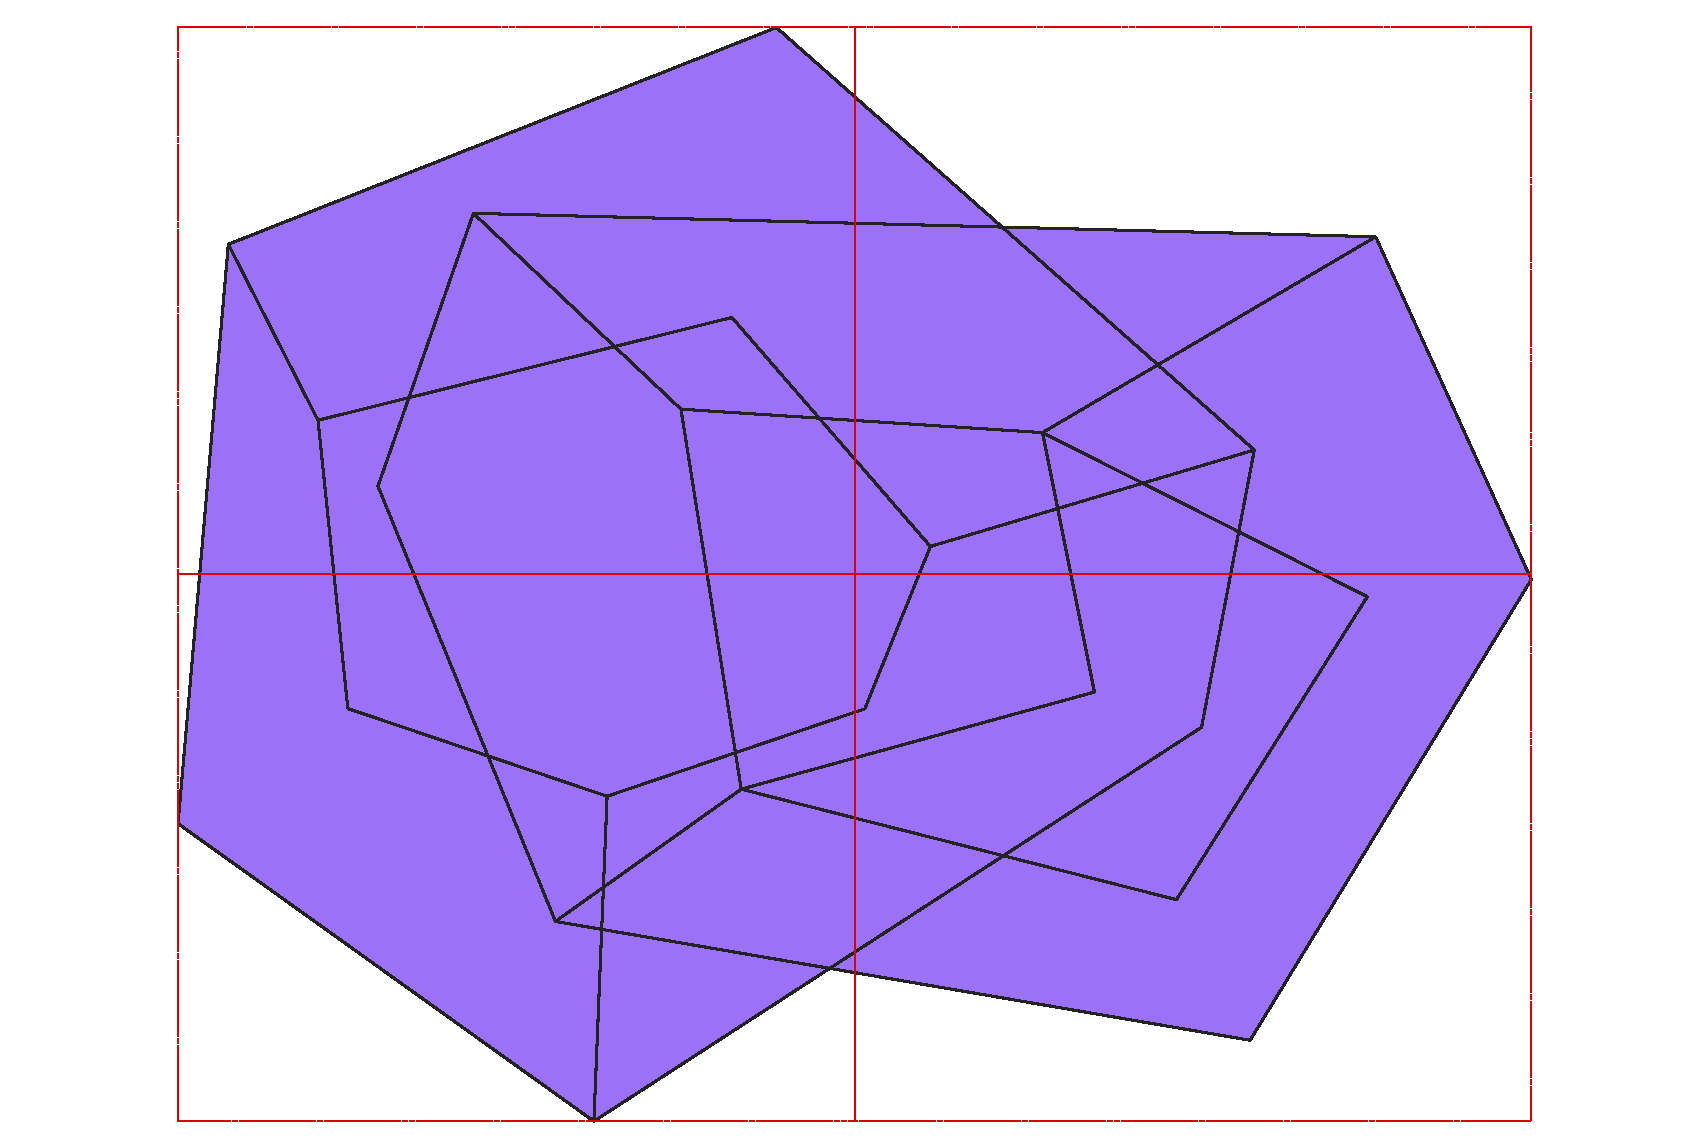
\includegraphics[width=0.8\linewidth]{figures/DCEL02_partitions} 
\end{frame}

\begin{frame}{DCEL construction example}
    \centering 
    Clipping \\
    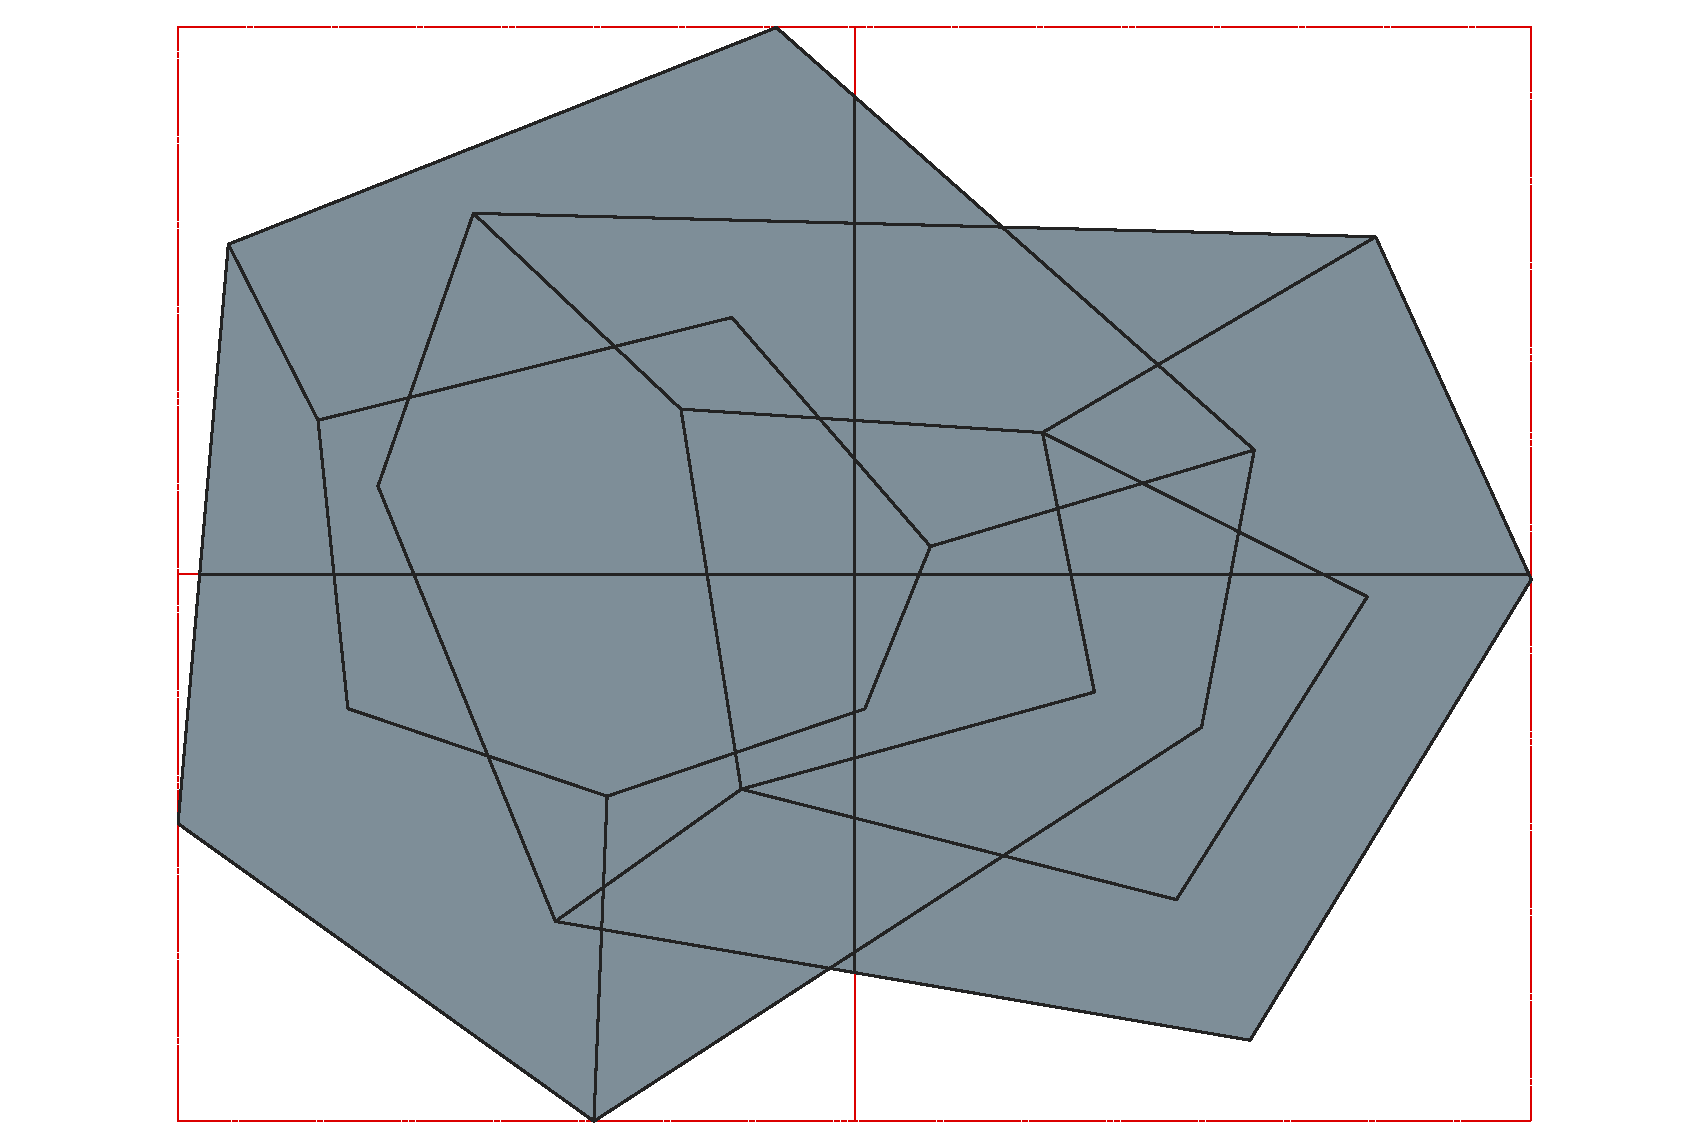
\includegraphics[width=0.8\linewidth]{figures/DCEL03_clipByPartition} 
\end{frame}

\begin{frame}{DCEL construction example}
    \centering 
    Local step input (set of clipped polygons) \\
    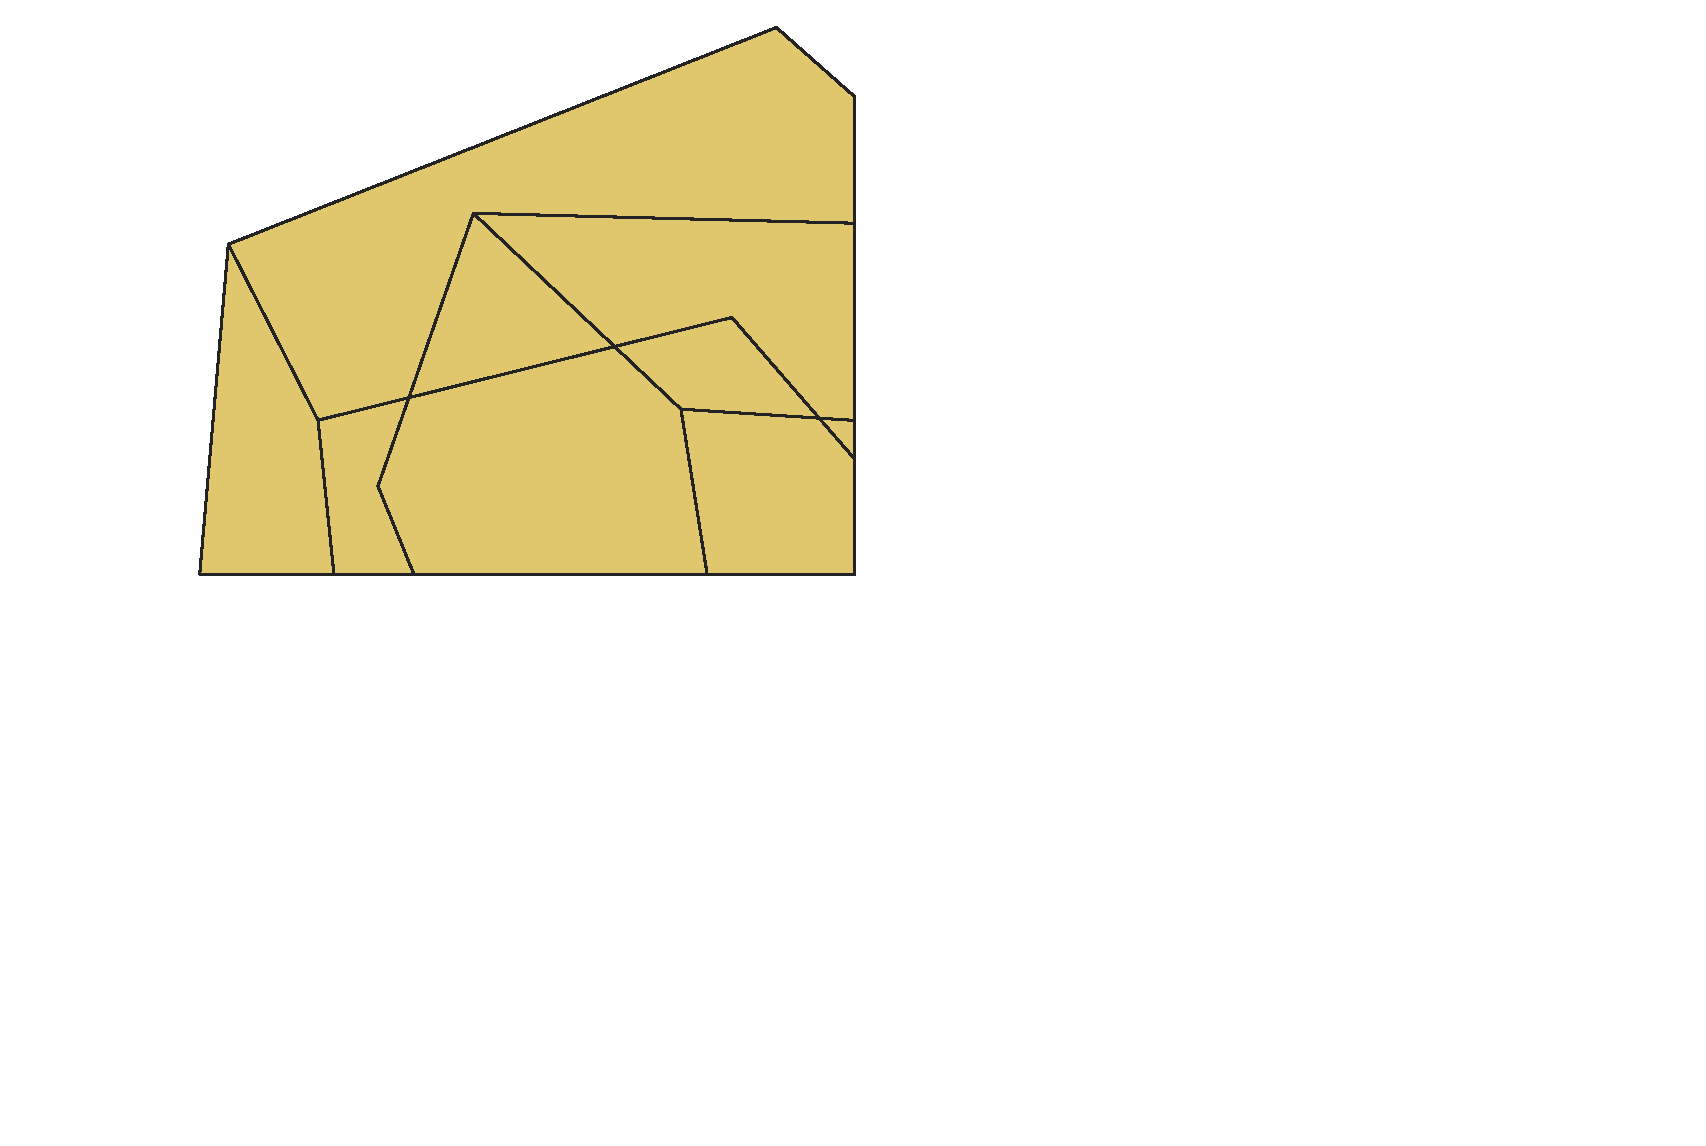
\includegraphics[width=0.8\linewidth]{figures/DCEL04_mapPartition} 
\end{frame}

\begin{frame}{DCEL construction example}
    \centering 
    Local step output (set of Half-edge records) \\
    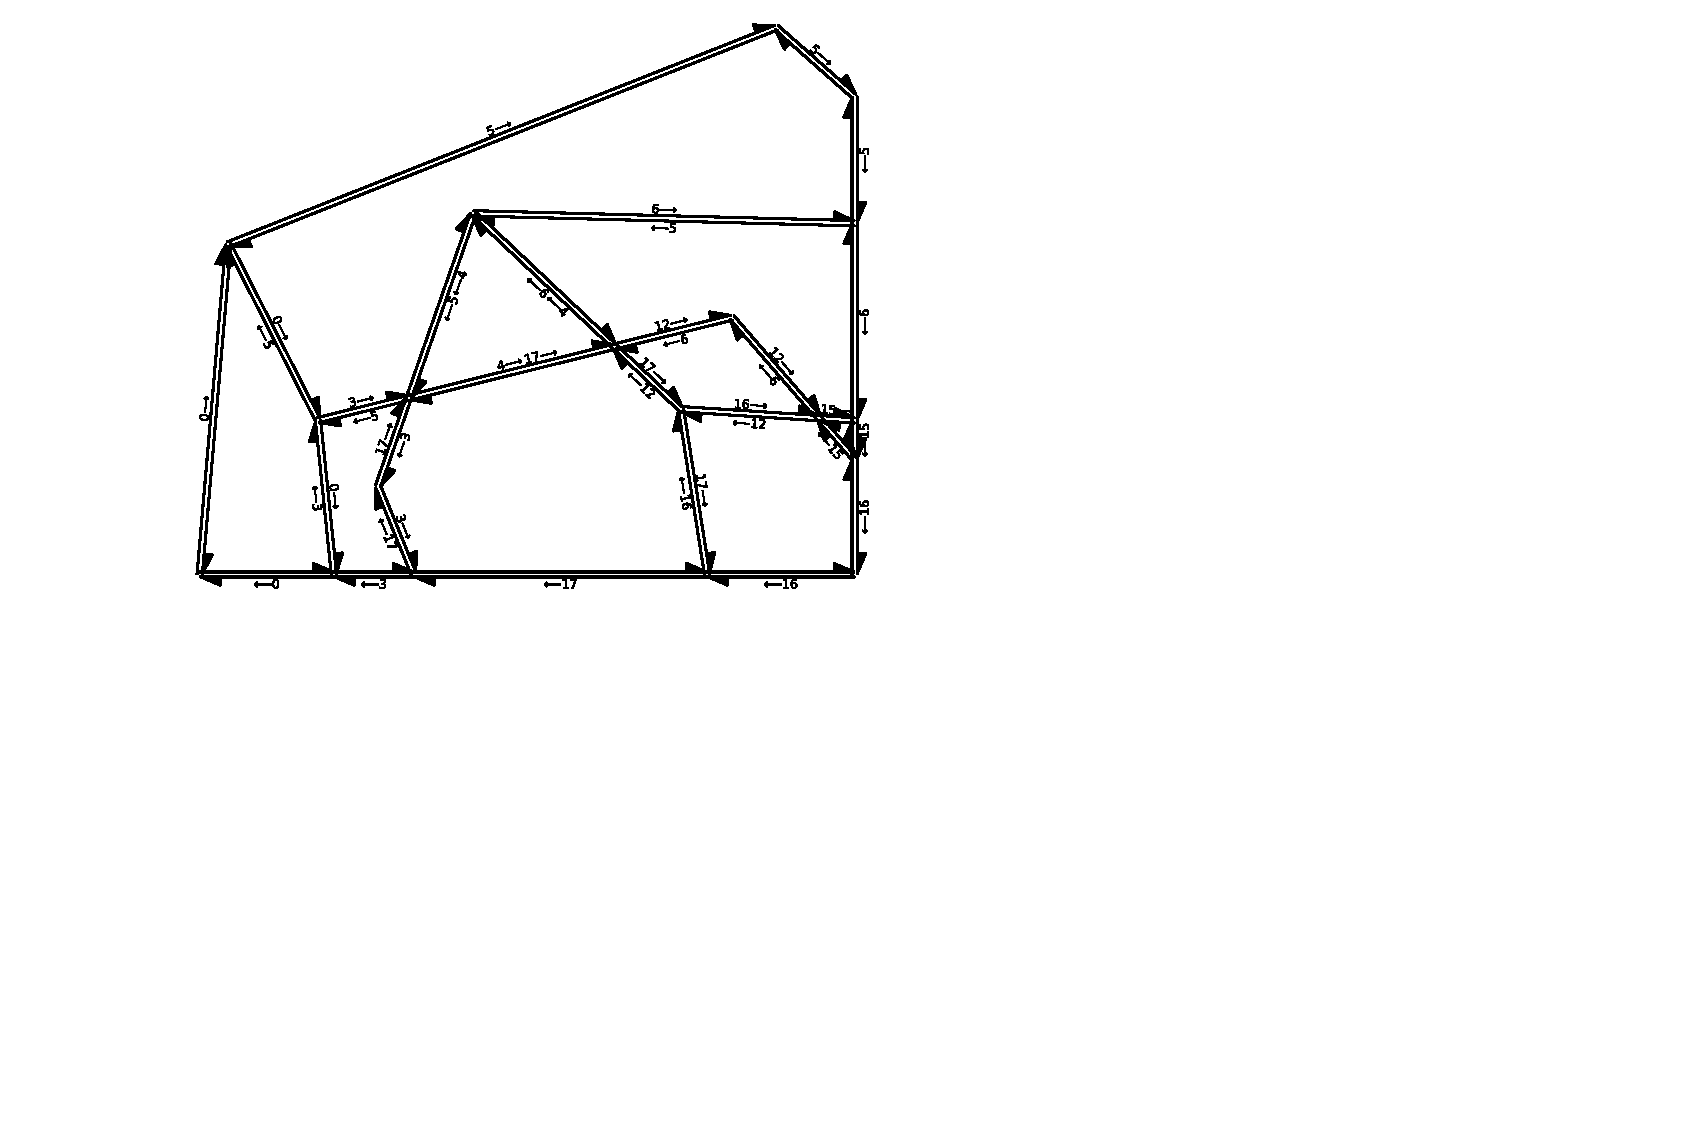
\includegraphics[width=0.8\linewidth]{figures/DCEL05_localDCEL} 
\end{frame}

\begin{frame}{DCEL construction example}
    \centering 
    Merge \\
    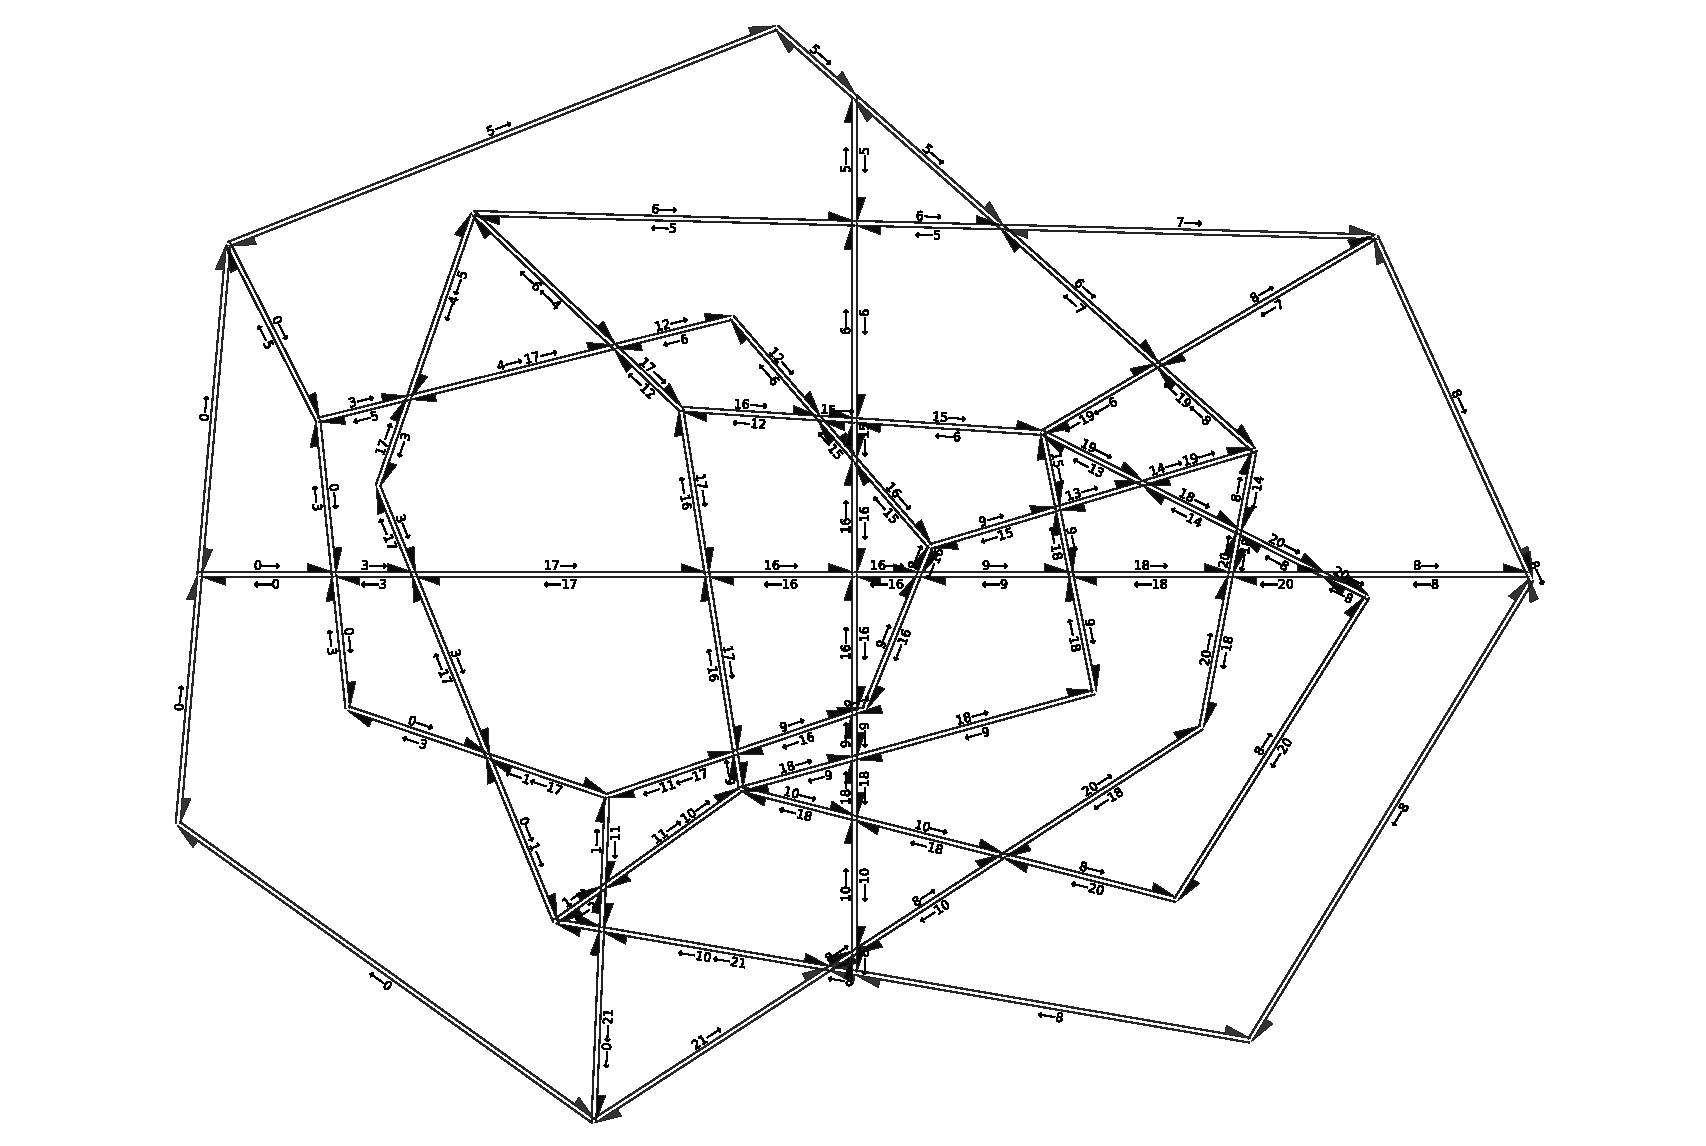
\includegraphics[width=0.8\linewidth]{figures/DCEL06_Merge} 
\end{frame}

\end{document}
